\documentclass[11pt]{article}
\usepackage[BoldFont,SlantFont,CJKchecksingle]{xeCJK}
\usepackage[top=0.5in,bottom=0.5in,left=1.25in,right=0.8in]{geometry}
\setCJKmainfont[BoldFont=SimHei]{SimSun}
\setCJKmonofont{SimSun}% 设置缺省中文字体
\parindent 0em   %段首缩进
%\usepackage{indentfirst}	%设置第一段也首行缩进
\linespread{1}	%设置行距
\addtolength{\parskip}{.4em}	%增加段间距0.4em
\usepackage{amsmath} % 插入数学公式
\usepackage[colorlinks,linkcolor=blue]{hyperref} 	%设置超链接

% 设置页眉页脚
\usepackage{fancyhdr}
\pagestyle{fancy}
\lhead{} 
\chead{} 
\rhead{\bfseries {ramayzhu0625@gmail.com}} 
\lfoot{} 
\cfoot{}
\rfoot{\thepage} 
\renewcommand{\headrulewidth}{0.4pt} 
\renewcommand{\footrulewidth}{0.4pt}

% \includegraphics[width = .8\textwidth]{pic.png}  图片的宽度会被缩放至页面宽度的百分之八十,图片的总高度会按比例缩放 

\begin{document}
	\title{Machine Learning Week-4}
	\author{ramay7}
	
	\maketitle % 显示标题
	\tableofcontents % 生成目录
	%\newpage
	
	\section{Neural Network}
		If network has $s_j$ units in layer $j$, $s_{j+1}$ units in layer $j+1$, then $\theta^{(j)}$ will be of dimension $s_{j+1} \times (s_j + 1)$. The +1 comes from the addition in $\theta^{(j)}$ for the 'bias nodes', $x_0$ and $\theta_{0}^{(j)}$. The 'bias unit' is always equal to 1. For instance, consider a three layer neural network with two inputs, 4 hidden units, and one output unit, the dimension of $\theta^{(1)}$ is 4 by 3 (4 $\times$ 3).
		
		In neural networks, we use the same logistic function as in classification($\frac{1}{1+e^{-\theta^{T}X}}$), yet we sometimes call it sigmoid(logistic) function. In this situation, our 'theta' parameters are sometimes called 'weights'.
		
		We can have intermediate layers of nodes between the input and output layers called the 'hidden layers'.
		
		Let's set:
		
		$$Z^{(j)} = \theta^{(j-1)}a^{(j-1)}$$
		we are multiplying our matrix $\theta^{(j-1)}$ with dimentions $s_j \times (n+1)$ (where $s_j$ is the number of our activation nodes) by our vector $a^{(j-1)}$ with height (n+1). This gives us our vector $Z^{(j)}$ with height $s_j$. Now we can get a vector of our activation nodes for layer j as follows:
		
		$$a_{(j)} = g(z^{(j)})$$
		
	\section{Equation}
		
		$$
		\frac{\partial J}{\partial \theta_j} = \frac{1}{m} \sum_{i=1}^{m}((h_{\theta}(x^{(i)}) - y^{(i)})x_{j}^{(i)})
		$$
		
		$$
		\begin{aligned}
		\left[
			\begin{array}{c}
				\frac{\partial J}{\partial \theta_{0}}  \\
				\frac{\partial J}{\partial \theta_{1}}  \\
				\frac{\partial J}{\partial \theta_{2}}  \\
				.  \\
				.  \\
				.  \\
				\frac{\partial J}{\partial \theta_{n}}  
			\end{array}
		\right] 
		&= \frac{1}{m} 
		\left[
			\begin{array}{c}
			 \sum_{i=1}^{m}((h_{\theta}(x^{(i)}) - y^{(i)})x_{0}^{(i)} \\
		     \sum_{i=1}^{m}((h_{\theta}(x^{(i)}) - y^{(i)})x_{1}^{(i)}  \\
		     \sum_{i=1}^{m}((h_{\theta}(x^{(i)}) - y^{(i)})x_{2}^{(i)}  \\
		     .  \\
		     .  \\
		     .  \\
			 \sum_{i=1}^{m}((h_{\theta}(x^{(i)}) - y^{(i)})x_{n}^{(i)}  
			\end{array}
		\right] \\
		&= \frac{1}{m} \sum_{i=1}^{m}((h_{\theta}(X^{(i)}) - y^{(i)})X^{(i)} \\
		&= \frac{1}{m} X^{T}(h_{\theta}(X) - y)
		\end{aligned}
		$$
		
	\section{Simple Neural Network Application: XNOR}
	
	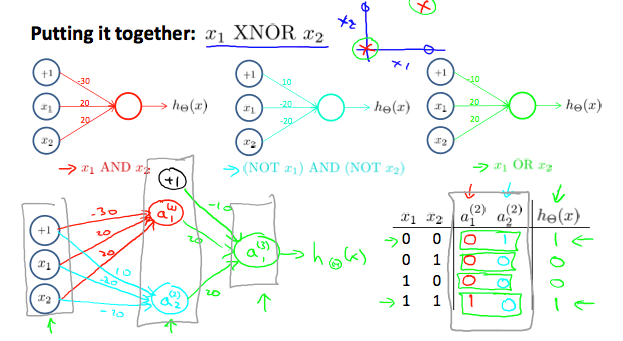
\includegraphics[width = .8\textwidth]{XNOR.png}
	
	\section{The End} 
		In this week's exercise, I have implemented one-vs-all logistic regression an neural networks to recognize hand-written digits. However, I don't know how to translate a picture into the form of a csv-file. Thanks to the original folder which contains a data set in ex3data1.mat that contains 5000 training examples of handwritten digits. Enjoy myself !

\end{document}